\section{Empirical Evaluation}
\label{section:evaluation}
Please showcase your empirical results in this section. Please clearly specify which sets of experiments of the original paper are considered in your report. Please also report the corresponding hyperparameters of each experiment.
\subsection{Lunar Lander Domain}
\subsection*{Experiment Results}
The paper's results:\\
\begin{center}
    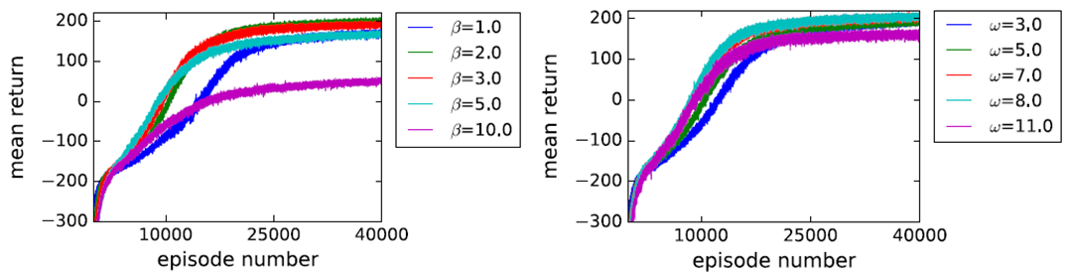
\includegraphics[scale=0.7]{lunar_paper1.png}\\
    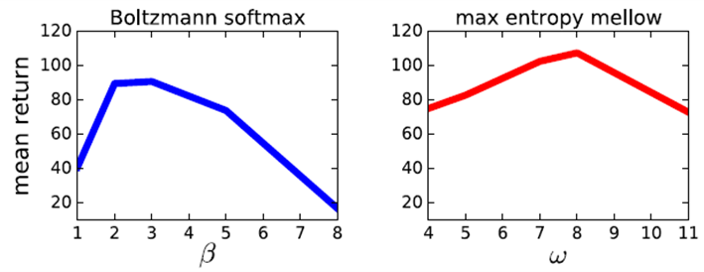
\includegraphics[scale=0.7]{lunar_paper2.png}
\end{center}
In the paper's results, the Boltzmann softsmax method performs well when $\beta=2, 3$, and the Mellowmax method 
performs well when $\omega=7, 8$.The Boltzmann softmax method, $\beta=10$ performs the worst in the 10 experiments, it 
gets a much lower average mean return than others.The Mellowmax method, $\omega=8$ performs the best in the 10 experiments.\\\\
Our results:\\
\begin{center}
    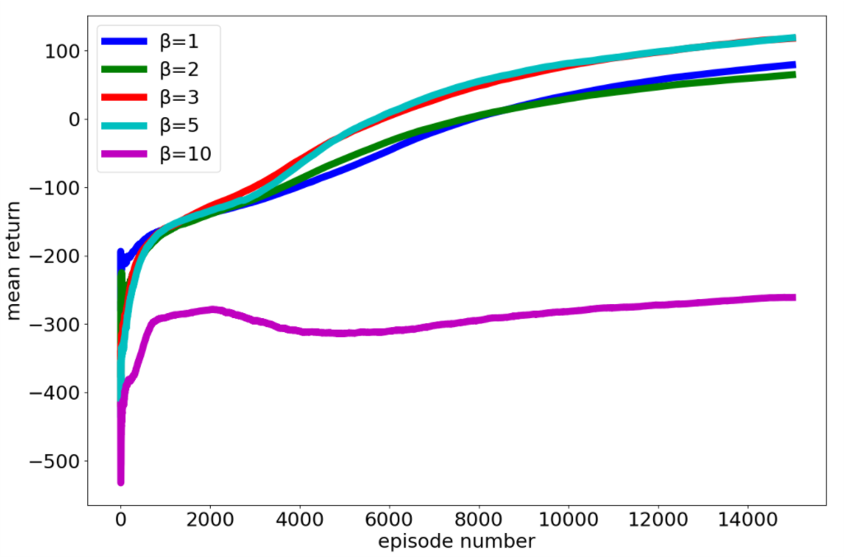
\includegraphics[scale=0.4]{lunar_rep1.png}
    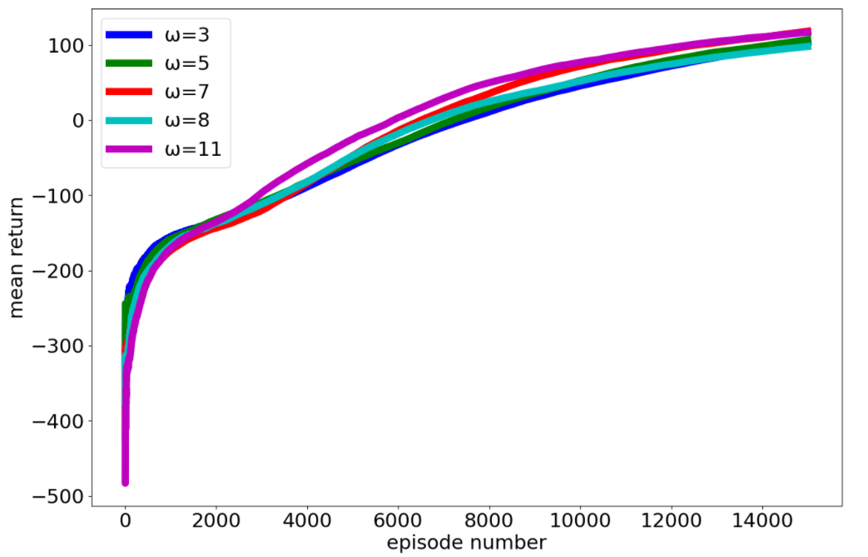
\includegraphics[scale=0.4]{lunar_rep2.png}\\
    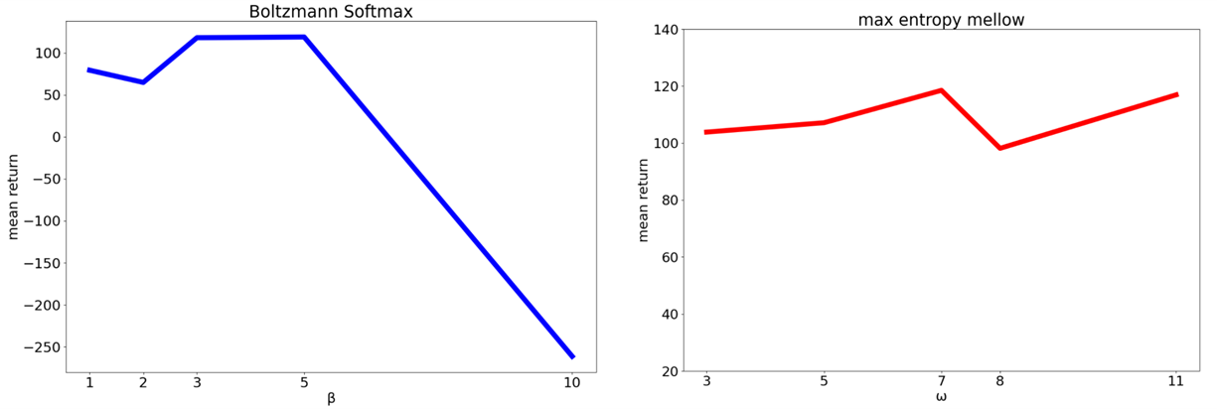
\includegraphics[scale=0.6]{lunar_rep3.png}
\end{center}
In our results, the Boltzmann softmax method performs well when $\beta=3, 5$, and the Mellowmax method 
performs well when $\omega=7, 11$. The Boltzmann softmax method, $\beta=10$ performs the worst in the 10 experiments and
gets a much lower average mean return than others. The Mellowmax method, $\omega=7$ performs the best in our 10 experiments.\\\\
\subsection*{Comparison}
Our experiment results are a little different from the paper's, and we think it is because that we use much less runs and less episodes in each run.
The mean return of Boltzmann softmax $\beta=10$ is about -300, and it's much lower than the paper's result. We find that it gets a lot of negative
 rewards at seed=22, its ewma reward is less than -1000 during almost all episodes, however, its ewma reward reaches 200 while seed=7654.
It seems that Boltzmann softmax $\beta=10$ is unstable, so the chosen seed affects a lots, and more runs are needed to get precise results.
